\chapter{Analisis}
\label{chap:analisis}
Bab ini berisi analisis yang digunakan pada skripsi ini, yaitu analisis Portal Akademik Mahasiswa 2018, analisis Portal Akademik Mahasiswa 2020, cara menerjemahkan perekaman kehadiran daring ke dalam selenium, analisis kebutuhan, dan analisis program sejenis.

\section{Analisis Portal Akademik Mahasiswa 2018}
\label{sec:pam} 
Portal Akademik Mahasiswa (selanjutnya disingkat dengan PAM) adalah sebuah \textit{web} yang di peruntukan bagi mahasiswa dalam rangka mendapatkan informasi kegiatan akademik mulai dari registrasi, melihat jadwal kuliah dan ujian, info nilai sampai pendaftaran sidang\cite{portalunpar}. Portal Akademik Mahasiswa dapat diakses melalui \url{https://studentportal.unpar.ac.id/}. 

\begin{figure}[H]
	\centering
	
\includegraphics[scale=0.4]{Gambar/halaman2018.jpg}
	\caption{Tampilan halaman awal Portal Akademik Mahasiswa} 
	\label{fig:studpor_home_2018}
\end{figure}

Pada Gambar \ref{fig:studpor_home_2018} adalah tampilan awal ketika masuk ke halaman \url{https://studentportal.unpar.ac.id/}. Mahasiswa perlu melakukan \textit{login} dengan \textit{email} dan \textit{password} mahasiswa UNPAR untuk dapat menggunakan fitur-fitur yang tersedia seperti:
\begin{enumerate}
	\item Fitur mengisi form rencana semester (FRS) atau melakukan perubahan rencana studi (PRS) secara online \\
	Panduan untuk melakukan FRS/PRS online.
	\begin{enumerate}
		\item Masuk ke halaman \url{https://studentportal.unpar.ac.id/} lalu klik tombol ``\textit{Login}'' yang dapat dilihat pada Gambar \ref{fig:studpor_home_2018}.
		\item Lakukan ``\textit{Login}'' dengan memasukan email dan password mahasiswa UNPAR pada halaman sso.
		\begin{figure}[H]
			\centering
			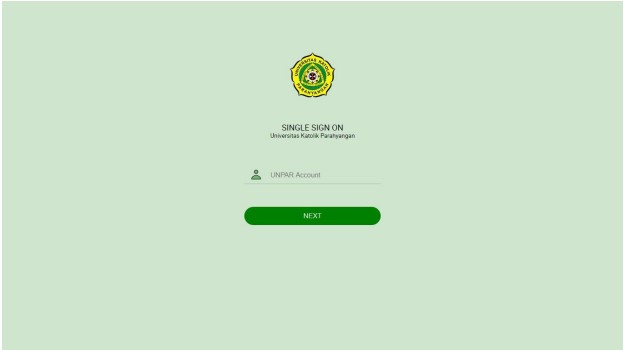
\includegraphics[scale=0.7]{Gambar/sso2018.jpg}
			\caption{Tampilan halaman untuk memasukan \textit{email} Portal Akademik Mahasiswa} 
			\label{fig:sso_2018}
		\end{figure}
		
		\begin{figure}[H]
			\centering
			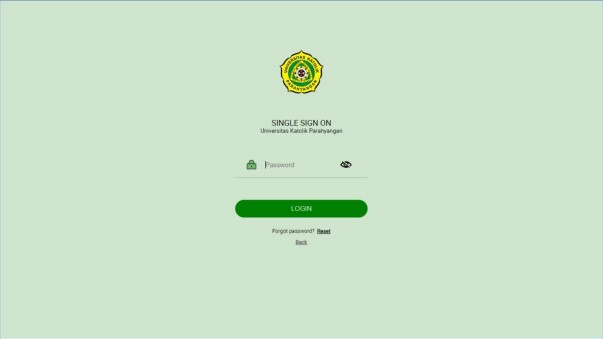
\includegraphics[scale=0.7]{Gambar/pass2018.jpg}
			\caption{Tampilan halaman untuk memasukan \textit{password} Portal Akademik Mahasiswa} 
			\label{fig:pass_2018}
		\end{figure}
		\item Ketika \textit{login} telah berhasil, maka browser akan menampilkan halaman utama, lalu klik pada heksagon berlabel `FRS/PRS' untuk melakukan FRS/PRS online.
		\begin{figure}[H]
			\centering
			
\includegraphics[scale=0.7]{Gambar/frs2018.jpg}
			\caption{Tampilan halaman utama} 
			\label{fig:frs_2018}
		\end{figure}
		\item Mahasiswa dapat melakukan FRS sesuai waktu yang sudah ditentukan atau mahasiswa dapat melakukan PRS setelah FRS selesai dan sesuai waktu yang sudah ditentukan untuk PRS.		
	\end{enumerate}
	
	\item Fitur Profil Mahasiswa
	\begin{enumerate}
		\item Mahasiswa melakukan \textit{login} terlebih dahulu. 
		\item Pada Gambar \ref{fig:frs_2018} terdapat menu ``PROFIL'' untuk menuju halaman profil mahasiswa. 
		\item Mahasiswa dapat melihat informasi data diri di halaman profil mahasiswa seperti pada Gambar \ref{fig:profil_2018}.
		\begin{figure}[H]
			\centering
			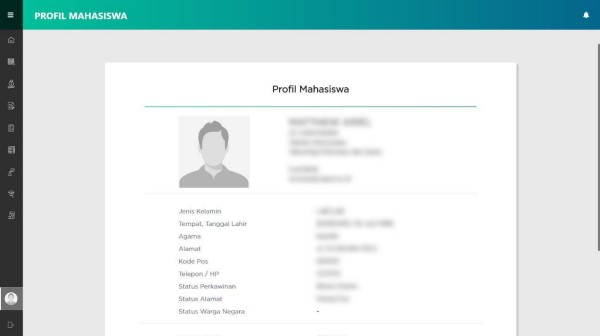
\includegraphics[scale=0.7]{Gambar/profil2018.jpg}
			\caption{Tampilan halaman profil mahasiswa} 
			\label{fig:profil_2018}
		\end{figure}
	\end{enumerate}
	
	\item Fitur Pembayaran
	\begin{enumerate}
		\item Mahasiswa melakukan \textit{login} terlebih dahulu. 
		\item Pada Gambar \ref{fig:frs_2018} terdapat menu ``PEMBAYARAN'' untuk menuju halaman pembayaran. 
		\item Pada halaman pembayaran, mahasiswa dapat melihat informasi pembayaran yang terdiri dari Tagihan Pembayaran, Riwayat Pembayaran, dan Keterangan.
	\end{enumerate}
	Pada Gambar \ref{fig:bayar_2018} adalah tabel ``Tagihan Pembayaran'' yang menampilkan jenis tagihan dan jumlah tagihan dari setiap jenis tagihan yang ada.
	\begin{figure}[H]
		\centering
		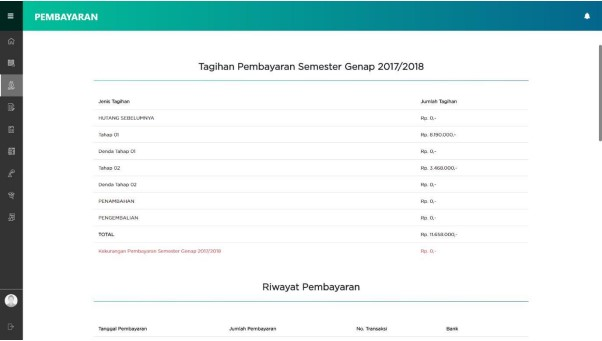
\includegraphics[scale=0.7]{Gambar/bayar2018.jpg}
		\caption{Tampilan halaman pembayaran bagian Tagihan Pembayaran} 
		\label{fig:bayar_2018}
	\end{figure}
	
	Pada Gambar \ref{fig:riw_2018} adalah tabel ``Riwayat Pembayaran'' yang menampilkan histori pembayaran yang telah dilakukan.
	\begin{figure}[H]
		\centering
		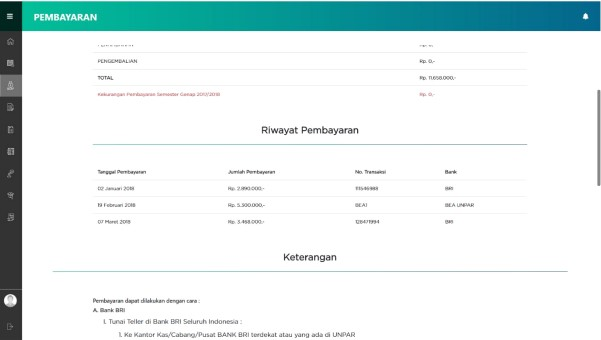
\includegraphics[scale=0.7]{Gambar/riwayat2018.jpg}
		\caption{Tampilan halaman pembayaran bagian Riwayat Pembayaran} 
		\label{fig:riw_2018}
	\end{figure}
	
	Pada Gambar \ref{fig:ketbayar_2018} adalah tabel ``Keterangan'' yang menampilkan tata cara pembayaran yang dapat dilakukan untuk melakukan pembayaran.
	\begin{figure}[H]
		\centering
		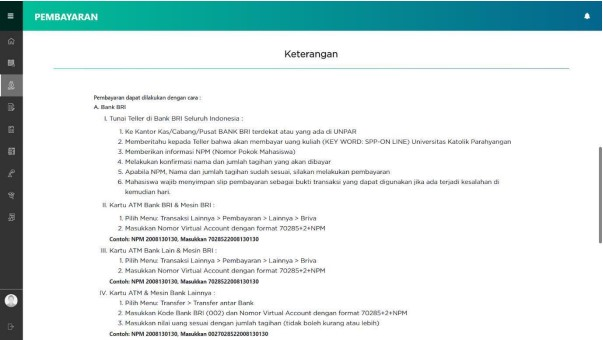
\includegraphics[scale=0.7]{Gambar/keterangan2018.jpg}
		\caption{Tampilan halaman pembayaran bagian Keterangan} 
		\label{fig:ketbayar_2018}
	\end{figure}
	\item Fitur Nilai
	Panduan untuk melihat informasi nilai mahasiswa.
	\begin{enumerate}
		\item Mahasiswa melakukan \textit{login} terlebih dahulu. 
		\item Menekan menu ``NILAI'' pada halaman setelah berhasil login seperti pada Gambar \ref{fig:frs_2018}. 
		\item Pada halaman nilai, mahasiswa dapat melihat informasi nilai dari setiap mata kuliah yang diambil.
		\begin{figure}[H]
			\centering
			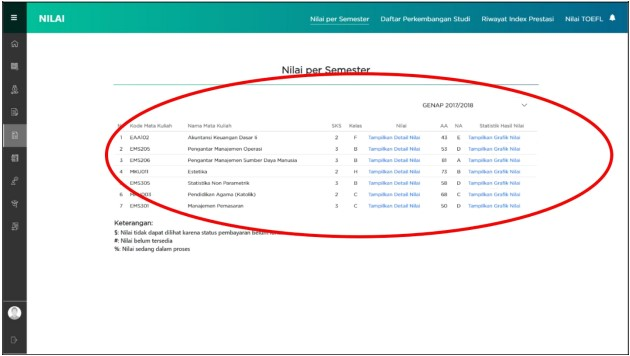
\includegraphics[scale=0.7]{Gambar/nilai2018.jpg}
			\caption{Tampilan halaman nilai bagian Nilai per Semester} 
			\label{fig:nilai_2018}
		\end{figure}
		\item Mahasiswa dapat mengakses menu ``Riwayat Index Prestasi'' untuk melihat `IPK' dan `IPS' mahasiswa.
		\begin{figure}[H]
			\centering
			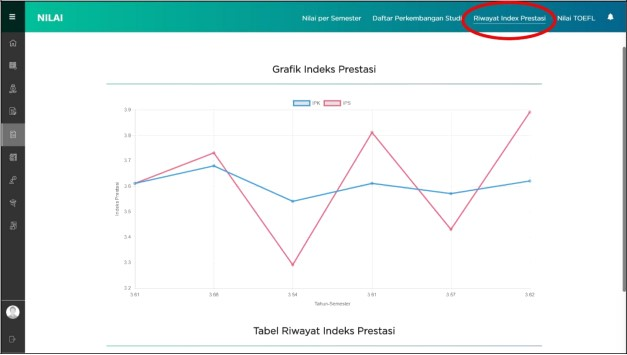
\includegraphics[scale=0.7]{Gambar/rip2018.jpg}
			\caption{Tampilan halaman nilai bagian Riwayat Index Prestasi} 
			\label{fig:rip_2018}
		\end{figure}
	\end{enumerate}	
\end{enumerate}
Portal Akademik Mahasiswa 2018 belum memiliki fitur perekaman kehadiran secara daring. Hal tersebut dikarenakan belum adanya pembelajaran secara daring, sehingga perekaman kehadiran dilakukan secara luring yang dimana perekaman kehadiran dilakukan secara langsung saat pembelajaran tatap muka.

\section{Analisis Portal Akademik Mahasiswa 2022}
\label{sec:alur} 
Portal Akademik Mahasiswa Universitas Katolik Parahyangan yang terbaru sejak 2020 sudah memiliki fitur perekaman kehadiran daring. Fitur tersebut dapat melakukan perekaman kehadiran secara daring untuk setiap mata kuliah yang diambil. 

Setiap mahasiswa sebelum memulai perkuliahan pada setiap mata kuliah perlu mengakses Portal Akademik Mahasiswa yang dapat diakses melalui \url{https://studentportal.unpar.ac.id/} seperti pada Gambar \ref{fig:studpor_home_2019}. 
\begin{figure}[H]
	\centering
	
\includegraphics[scale=0.225]{Gambar/halaman2019.jpg}
	\caption{Tampilan halaman awal Portal Akademik Mahasiswa} 
	\label{fig:studpor_home_2019}
\end{figure}

Setelah itu mahasiswa melakukan \textit{Login} dengan mengisi \textit{email} serta \textit{password} milik mahasiswa tersebut. Pada Gambar \ref{fig:login} merupakan tampilan untuk mengisi \textit{email} dan Gambar \ref{fig:pass} merupakan tampilan untuk mengisi \textit{password}.
\begin{figure}[H]
	\centering
	
\includegraphics[scale=0.225]{Gambar/login.jpg}
	\caption{Tampilan halaman Portal Akademik Mahasiswa untuk memasukan \textit{email}} 
	\label{fig:login}
\end{figure}

\begin{figure}[H]
	\centering
	
\includegraphics[scale=0.225]{Gambar/pass.jpg}
	\caption{Tampilan halaman Portal Akademik Mahasiswa untuk memasukan \textit{password}} 
	\label{fig:pass}
\end{figure}

Setelah berhasil melakukan \textit{login} akan ada dua kemungkinan yang terjadi pada halaman Portal Akademik Mahasiswa, yaitu pertama akan muncul notifkasi peringatan seperti pada Gambar \ref{fig:notif} dan kedua akan masuk langsung ke halaman utama Portal Akademik Mahasiswa seperti pada Gambar \ref{fig:jadwal}. Jika muncul notifikasi terlebih dahulu maka harus menutup notifikasi tersebut untuk dapat masuk ke halaman utama.
\begin{figure}[H]
	\centering
	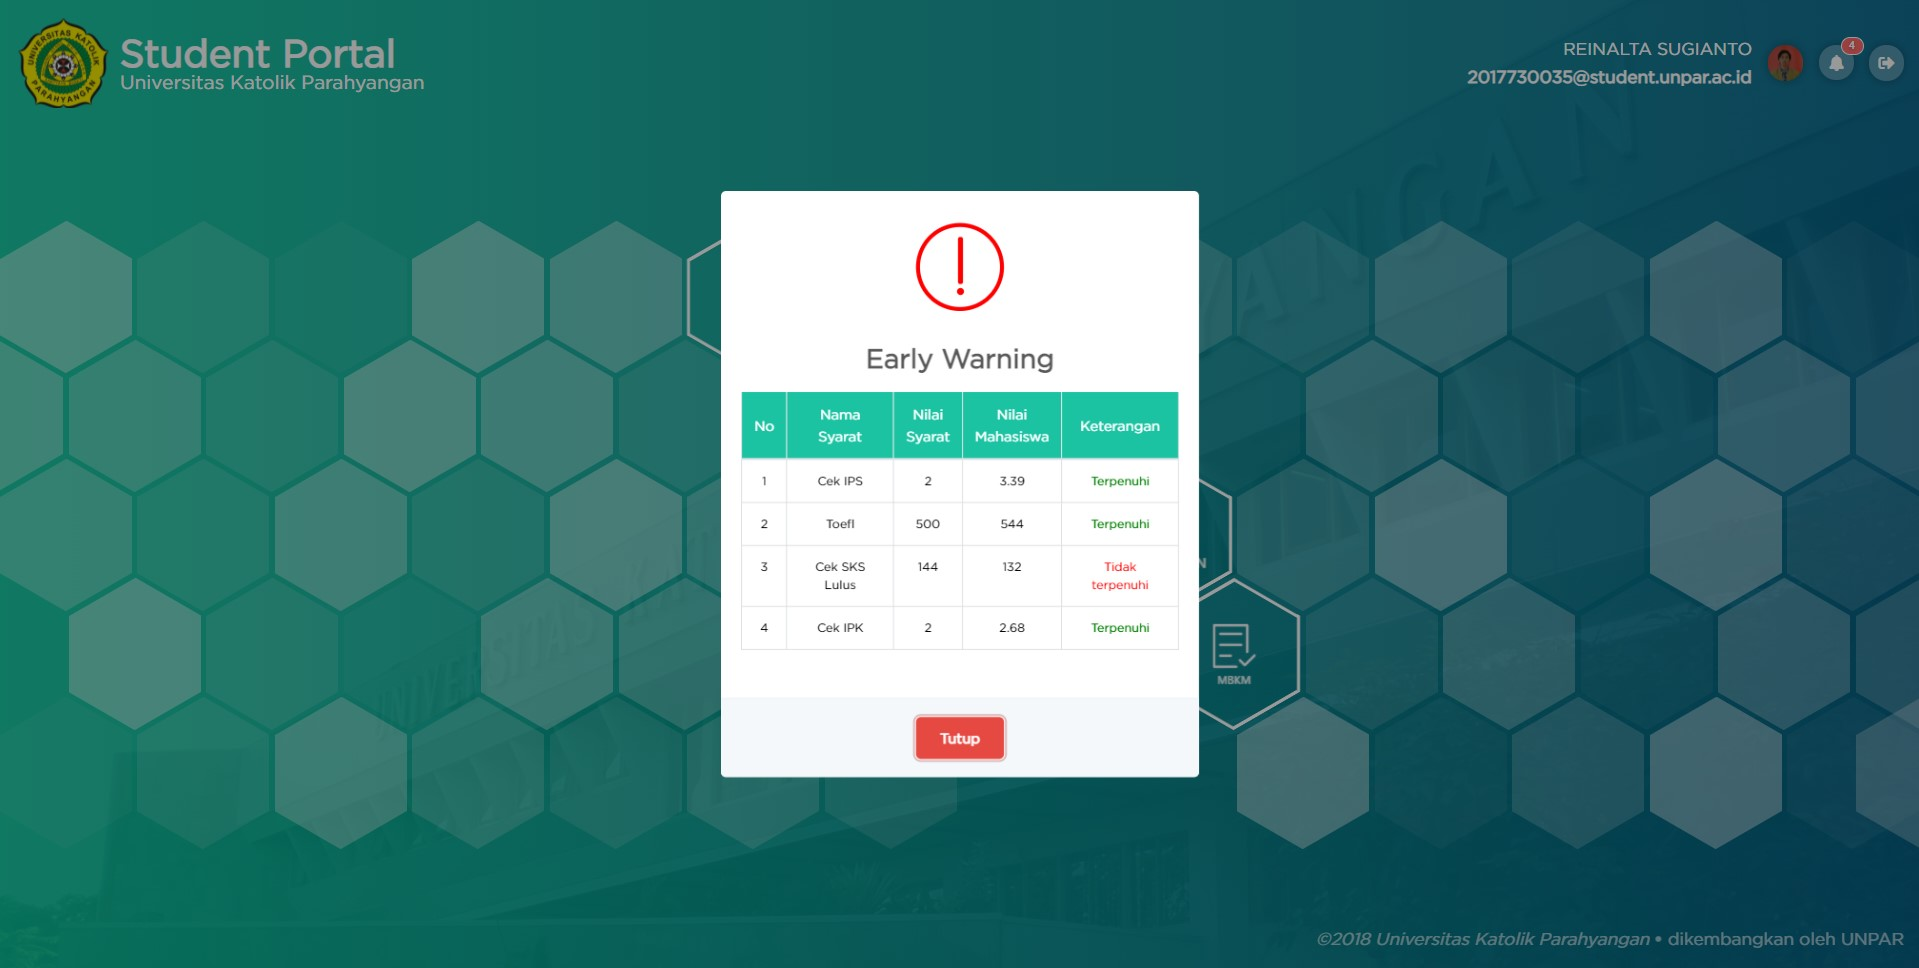
\includegraphics[scale=0.225]{Gambar/notif.jpg}
	\caption{Tampilan peringatan pada halaman Portal Akademik Mahasiswa} 
	\label{fig:notif}
\end{figure}

\begin{figure}[H]
	\centering
	
\includegraphics[scale=0.225]{Gambar/jadwal.jpg}
	\caption{Tampilan halaman Portal Akademik Mahasiswa setelah Berhasil \textit{Login}} 
	\label{fig:jadwal}
\end{figure}
	
Pada Gambar \ref{fig:notif} merupakan sebuah peringatan yang terkadang muncul menjelang berakhirnya suatu semester untuk melihat status kebutuhan mahasiswa untuk lulus, sehingga perlu menekan tombol ``Tutup'' terlebih dahulu untuk menekan tombol berbentuk heksagon ``JADWAL \& KEHADIRAN'' seperti pada Gambar \ref{fig:jadwal}. Jika tidak terjadi peringatan seperti pada  Gambar \ref{fig:notif}, maka dapat langsung menekan tombol berbentuk heksagon ``JADWAL \& KEHADIRAN'' seperti pada Gambar \ref{fig:jadwal}.

Setelah berhasil masuk ke halaman untuk perekaman kehadiran daring, mahasiswa perlu menekan tombol berwarna merah pada kolom bagian presensi pada tabel jadwal kehadiran mata kuliah (Gambar \ref{fig:absen}). 	
\begin{figure}[H]
	\centering
	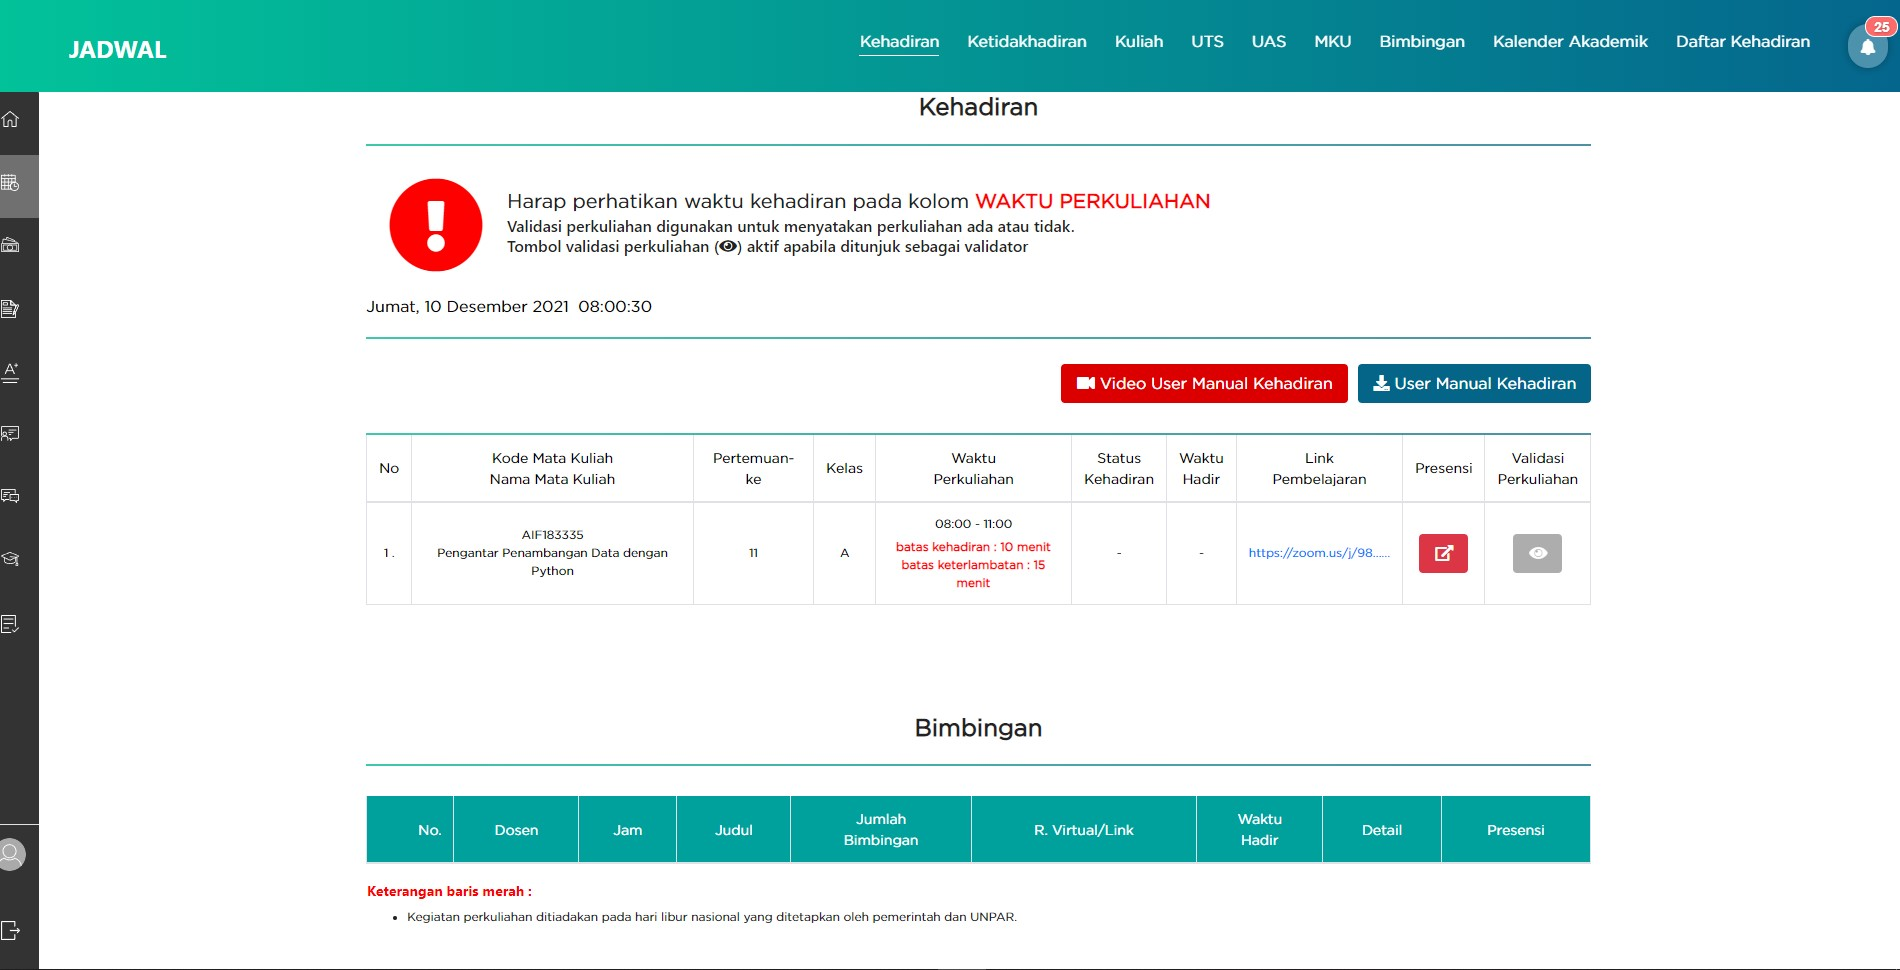
\includegraphics[scale=0.225]{Gambar/absen.jpg}
	\caption{Tampilan halaman Portal Akademik Mahasiswa untuk Melakukan Absen} 
	\label{fig:absen}
\end{figure}

Setelah mengklik tombol presensi maka akan muncul notifikasi bahwa absensi telah berhasil dan mahasiswa perlu menekan tombol ``OK''. 
\begin{figure}[H]
	\centering
	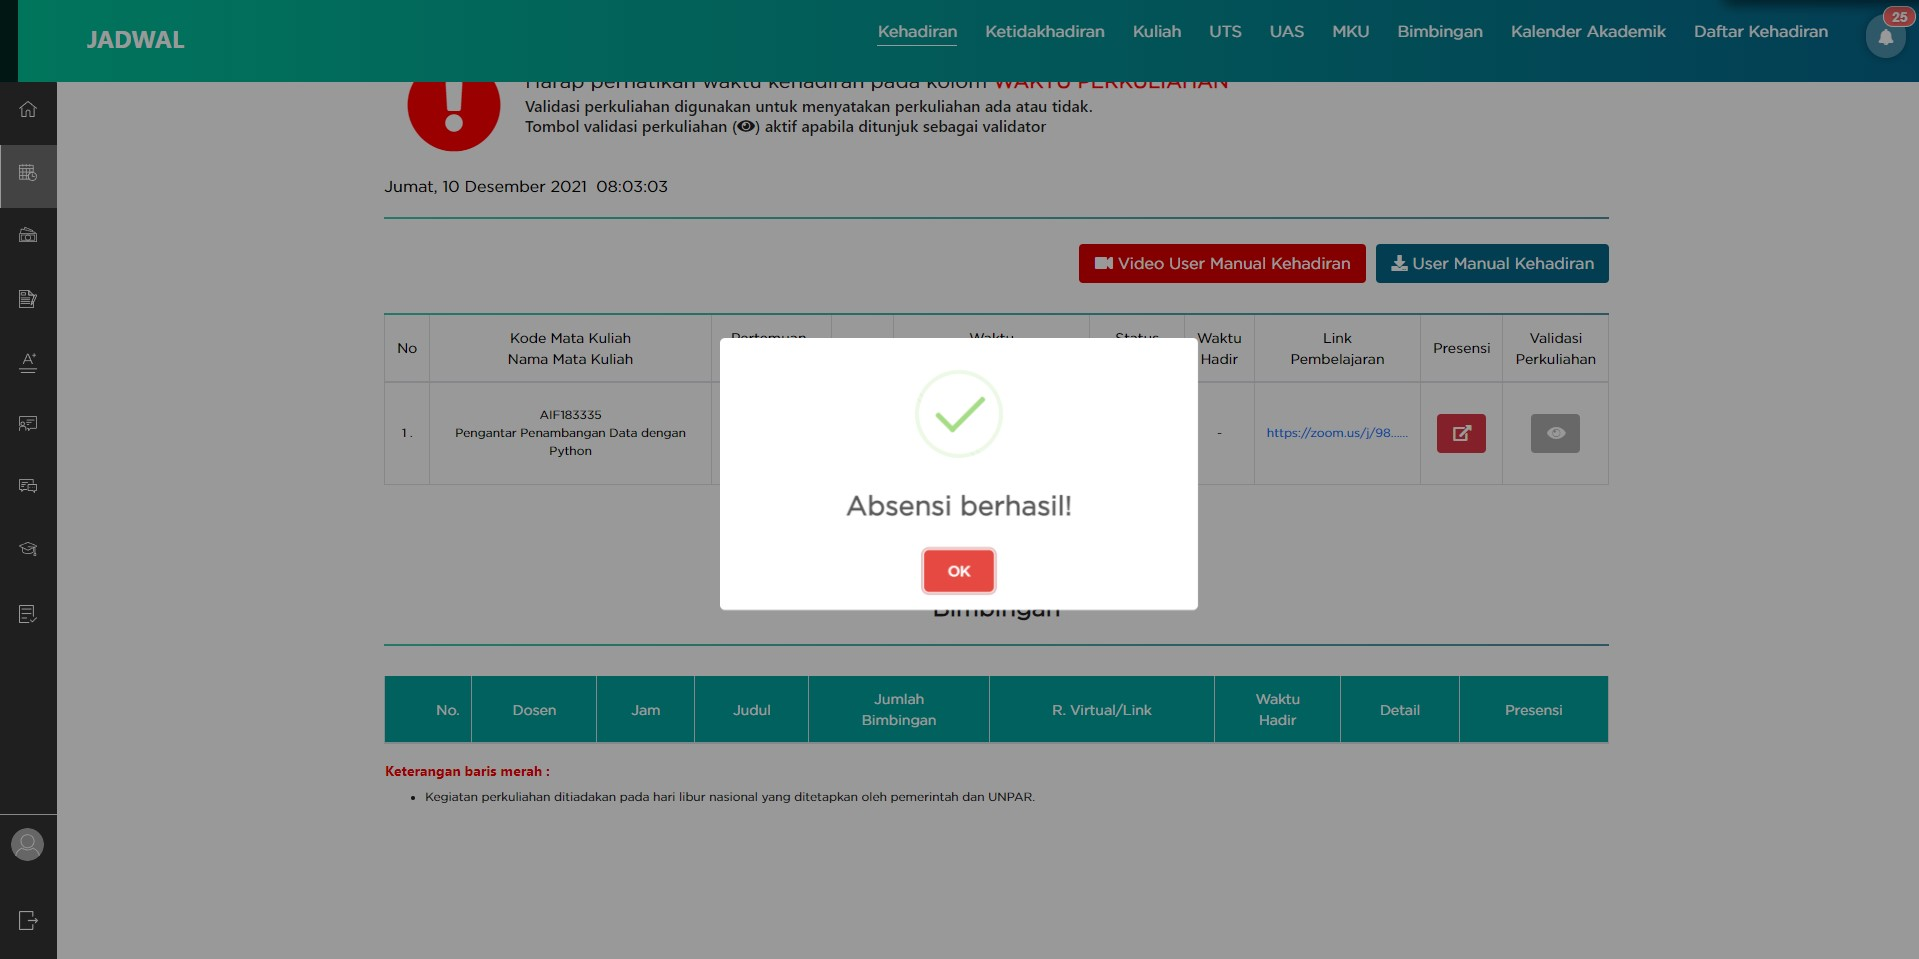
\includegraphics[scale=0.225]{Gambar/berhasilAbsen.jpg}
	\caption{Tampilan Pemberitahuan Absensi Berhasil} 
	\label{fig:berhasil}
\end{figure}

\section{Cara Menerjemahkan Perekaman Kehadiran Daring ke dalam Selenium}
\label{sec:terjemah} 
Otomatisasi perekaman kehadiran online ini akan menggunakan selenium, sehingga perlu diterjemahkan dari cara perekaman kehadiran online secara normal ke dalam selenium. Membuka situs web \url{https://studentportal.unpar.ac.id/} menggunakan selenium adalah dengan menggunakan \textit{method get()}. Setiap tombol yang ingin ditekan akan diambil elemennya agar dapat diotomatisasikan dengan selenium. Pada \textit{browser} Google Chrome, cara mendapatkan setiap elemen yang dibutuhkan adalah dengan melakukan \textit{inspect} elemen pada bagian yang ingin diambil elemennya. Elemen yang ingin diambil dapat dilakukan dengan berbagai macam cara seperti yang sudah dijelaskan pada Bab \ref{sec:selenium}. Beberapa faktor yang dapat dijadikan acuan untuk memilih cara dalam mengambil elemen dapat dilihat dari sebagai berikut:
\begin{enumerate}
	\item Sederhana \\
	Semakin pendek penulisan \textit{query selector} semakin baik dan stabil, misalnya mengambil elemen dengan \textit{CSS selector} yang namanya ``\#username''.
	\item Mudah dimengerti dan dibaca \\
	Menulis \textit{query selector} yang mudah dibaca dan dimengerti sehingga lebih mudah untuk dipahami, contohnya ``\#login-button'' yang artinya memilih elemen tombol untuk \textit{login}. Tidak disarankan menulis \textit{query selector} yang panjang atau sulit dibaca, contohnya mengambil elemen dengan cara XPath seperti yang sudah ditulis pada Bab \ref{sec:selenium} dengan kode program \ref{kode:2:elemenxpath}.
\end{enumerate}
Pemilihan cara pengambilan elemen yang diutamakan adalah dengan mengambil elemen berdasarkan \textit{CSS selector}, tetapi tidak menutup kemungkinan menggunakan cara yang lain untuk menemukan suatu elemen. Jika mengambil elemen berdasarkan \textit{CSS selector} tidak perlu khawatir jika struktur HTML diubah, karena \textit{CSS selector} sangat jarang diubah saat melakukan pembaharuan pada suatu situs web. 
Dalam melakukan otomatisasi perekaman kehadiran online pasti perlu memasukan \textit{email} dan \textit{password}, sehingga untuk memasukan hal tersebut perlu menggunakan \textit{method sendKeys()}. Memasukan \textit{email} dan \textit{password} ini tidak langsung dimasukan ke dalam programnya, tetapi melalui file konfigurasi yang diisi \textit{email} dan \textit{password}, lalu dipanggil ke kode programnya. 

\section{Analisis Kebutuhan}
Pada subbab ini akan dijelaskan mengenai analisis kebutuhan yang diperlukan untuk membuat program perekaman kehadiran daring otomatis. Analisis kebutuhan ini berasal dari analisis hasil survei perekaman kehadiran daring dan luring.

\subsection{Analisis Hasil Survei Perekaman Kehadiran Daring dan Luring}
\label{sec:survei} 
Survei perekaman kehadiran daring dan luring dilakukan untuk mengetahui berapa lama waktu yang dibutuhkan untuk melakukan perekaman kehadiran secara daring maupun luring dan beberapa informasi dalam melakukan perekaman kehadiran daring. Survei ini diberikan kepada mahasiswa dan dosen Teknik Informatika Universitas Katolik Parahyangan. Hasil survei menunjukan bahwa waktu yang dibutuhkan untuk perekaman kehadiran secara luring lebih cepat bagi para mahasiswa maupun dosen dibandingkan waktu yang dibutuhkan untuk perekaman kehadiran secara daring.

\subsubsection{Hasil Survei Mahasiswa}
Berdasarkan hasil survei yang telah diterima dari 21 orang responden yang merupakan mahasiswa Teknik Informatika Universitas Katolik
Parahyangan yang terdiri dari mahasiswa angkatan 2017 sampai 2019, dengan pertanyaan yang diajukan kepada responen dan rangkuman jawaban hasil survei sebagai berikut:
\begin{enumerate}
	\item \textbf{Berapa detik perkiraan waktu interaksi yang Anda butuhkan untuk melakukan perekaman kehadiran daring di \url{https://studentportal.unpar.ac.id/}, mulai dari membuka \textit{browser}, lalu masuk ke \url{https://studentportal.unpar.ac.id/}, lalu mengklik tombol presensi?}
	\begin{figure}[H]
		\centering
		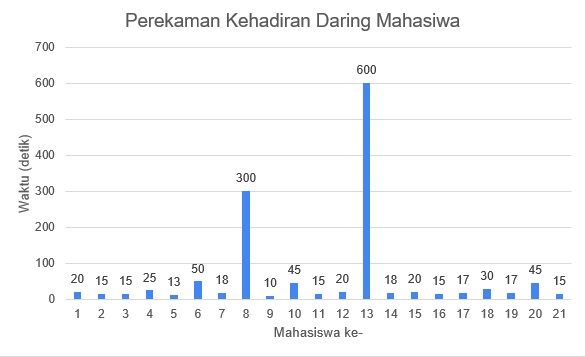
\includegraphics[scale=0.6]{Gambar/DaringMahasiswa.jpg}
		\caption{Histogram Waktu Perekaman Kehadiran Daring Mahasiswa} 
		\label{fig:DaringMahasiswa}
	\end{figure}
	Pada Gambar \ref{fig:DaringMahasiswa} merupakan visualisasi dari hasil survei mengenai lama waktu yang dibutuhkan dari 21 mahasiswa untuk melakukan perekaman kehadiran secara daring. Histogram ini dikelompokan berdasarkan rentang waktu per 20 detik. Histogram tersebut menunjukan bahwa mayoritas mahasiswa sebanyak 14 orang memiliki rentang waktu mulai dari 0 sampai 20 detik melakukan perekaman kehadiran secara daring, sebanyak 2 orang memilik rentang waktu 21 sampai 40 detik, 3 orang memiliki rentang waktu 41 sampai 60 detik, dan 2 orang memiliki rentang waktu di atas 100 detik. Hasil survei perekeman kehadiran secara daring untuk setiap mahasiswa secara jelas dapat dilihat pada tabel \ref{tab:daringMahasiswa}. Jawaban dari 21 orang responden adalah mulai dari waktu paling cepat 10 detik hingga waktu paling lama 600 detik.
	\begin{table}[ht]			
		\caption{Tabel Perekaman Daring Mahasiswa}
		\centering
		\begin{tabular}{|p{4cm} |p{7cm}|}\hline
			Jumlah Responden &  Waktu Perekaman Kehadiran Daring \\ \hline     
			1 orang &  10 detik\\ \hline 
			1 orang &  13 detik\\ \hline 
			5 orang &  15 detik\\ \hline 
			2 orang &  17 detik\\ \hline 
			2 orang &  18 detik\\ \hline 
			3 orang &  20 detik\\ \hline
			1 orang &  25 detik\\ \hline 
			1 orang &  30 detik\\ \hline 
			2 orang &  45 detik\\ \hline
			1 orang &  50 detik\\ \hline 
			1 orang &  300 detik\\ \hline 
			1 orang &  600 detik\\ \hline		
		\end{tabular}
		\label{tab:daringMahasiswa}
	\end{table}\\
	Jika dihitung rata-rata waktu yang dibutuhkan untuk melakukan perekaman kehadiran daring bagi para mahasiswa adalah 63 detik.
	\newpage
	\item \textbf{Berapa detik perkiraan waktu interaksi yang Anda butuhkan untuk melakukan perekaman kehadiran luring menggunakan metode tanda tangan seperti pembelajaran di kelas, mulai dari mengambil kertas absen, lalu tanda tangan, lalu memberikannya ke rekan di sebelah anda?}
	\begin{figure}[H]
		\centering
		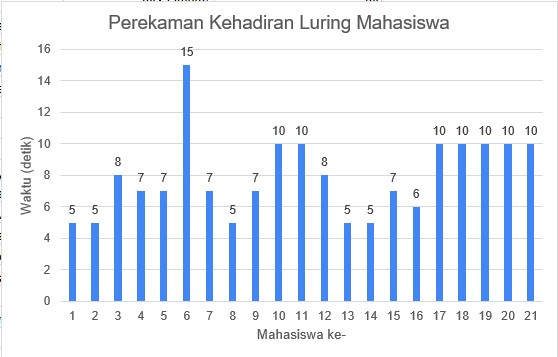
\includegraphics[scale=0.7]{Gambar/LuringMahasiswa.jpg}
		\caption{Histogram Waktu Perekaman Kehadiran Luring Mahasiswa} 
		\label{fig:LuringMahasiswa}
	\end{figure}
	Pada Gambar \ref{fig:LuringMahasiswa} merupakan visualisasi dari hasil survei mengenai lama waktu yang dibutuhkan dari 21 mahasiswa untuk melakukan perekaman kehadiran secara luring. Histogram ini dikelompokan berdasarkan rentang waktu per 20 detik. Histogram tersebut menunjukan bahwa seluruh mahasiswa sebanyak 21 orang memiliki rentang waktu mulai dari 0 sampai 20 detik melakukan perekaman kehadiran secara daring. Hasil survei perekeman kehadiran secara luring untuk setiap mahasiswa secara jelas dapat dilihat pada tabel \ref{tab:luringMahasiswa}. Jawaban dari 21 orang responden adalah mulai dari waktu paling cepat 5 detik hingga waktu paling lama 15 detik.
	 \begin{table}[ht]			
	  	\caption{Tabel Perekaman Luring Mahasiswa}
	  	\centering
	  	\begin{tabular}{|p{4cm} |p{7cm}|}\hline
	  		Jumlah Responden &  Waktu Perekaman Kehadiran Luring \\ \hline     
	  		5 orang &  5 detik\\ \hline 
	  		1 orang &  6 detik\\ \hline 
	  		5 orang &  7 detik\\ \hline 
	  		2 orang &  8 detik\\ \hline 
	  		7 orang &  10 detik\\ \hline 
	  		1 orang &  15 detik\\ \hline
	  	\end{tabular}
	  	\label{tab:luringMahasiswa}
	 \end{table}\\
	Jika dihitung rata-rata waktu yang dibutuhkan untuk melakukan perekaman kehadiran luring bagi para mahasiswa adalah 7,95 detik.
\end{enumerate}
Berdasarkan hasil survei terdapat beberapa informasi yang dirasakan mahasiswa ketika dalam melakukan perekaman kehadiran daring. Faktor yang menjadi kendala dalam melakukan perekaman kehadiran daring bagi mahasiswa, sebagai berikut:
\begin{enumerate}
	\item Faktor waktu berpengaruh pada kecepatan dalam melakukan perekaman kehadiran daring. Perkuliahan mahasiswa pada jam-jam padat, seperti jam 7 pagi, 9 pagi, 12 siang, atau 1 siang ini biasanya mahasiswa akan mengalami kendala waktu yang lama untuk dapat melakukan perekaman kehadiran daring.
	\item Faktor internet berpengaruh pada kecepatan dalam perekaman kehadiran daring. Setiap mahasiswa pasti menggunakan internet dari provider yang berbeda sehingga waktu yang dibutuhkan dalam melakukan perekaman kehadiran daring bergantung pada internet yang digunakan oleh mahasiswa.
\end{enumerate}

Kesimpulan dari hasil survei mahasiswa menunjukan bahwa rata-rata waktu yang dibutuhkan secara luring adalah 7,95 detik lebih cepat dibandingkan dengan rata-rata waktu yang dibutuhkan secara daring adalah 63 detik.

\subsubsection{Hasil Survei Dosen}
Berdasarkan hasil survei yang telah diterima dari 6 orang responden yang merupakan dosen Teknik Informatika Universitas Katolik Parahyangan, dengan pertanyaan yang diajukan kepada responen dan rangkuman jawaban hasil survei sebagai berikut:
\begin{enumerate}
	\item \textbf{Berapa detik perkiraan waktu interaksi yang Anda butuhkan untuk melakukan perekaman kehadiran daring di \url{https://akuhadir.unpar.ac.id} ?}
	\begin{figure}[H]
		\centering
		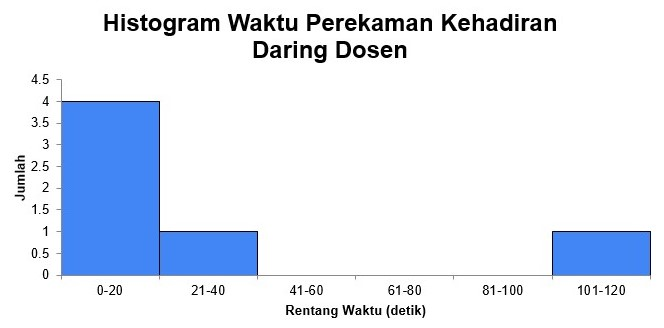
\includegraphics[scale=0.7]{Gambar/DaringDosen.jpg}
		\caption{Histogram Waktu Perekaman Kehadiran Daring Dosen} 
		\label{fig:DaringDosen}
	\end{figure}
	Pada Gambar \ref{fig:DaringDosen} merupakan visualisasi dari hasil survei mengenai lama waktu yang dibutuhkan dari 6 dosen untuk melakukan perekaman kehadiran secara daring. Histogram ini dikelompokan berdasarkan rentang waktu per 20 detik. Histogram menunjukan bahwa sebanyak 4 dosen memiliki rentang waktu 0 sampai 20 detik, 1 dosen memiliki rentang waktu 21 sampai 40 detik, dan 1 dosen memiliki rentang waktu 101 sampai 120 detik. Hasil survei perekeman kehadiran daring untuk setiap dosen secara jelas dapat dilihat pada tabel \ref{tab:daringDosen}.
	\begin{table}[ht]			
		\caption{Tabel Perekaman Daring Dosen}
		\centering
		\begin{tabular}{|p{4cm} |p{7cm}|}\hline
			Jumlah Responden &  Waktu Perekaman Kehadiran Daring \\ \hline     
			1 orang &  1 detik\\ \hline 
			1 orang &  10 detik\\ \hline 
			2 orang &  15 detik\\ \hline 
			1 orang &  30 detik\\ \hline 
			1 orang &  120 detik\\ \hline 
		\end{tabular}
		\label{tab:daringDosen}
	\end{table}\\
	Jika dihitung rata-rata waktu yang dibutuhkan untuk melakukan perekaman kehadiran daring bagi para dosen adalah 31,83 detik.

	\item \textbf{Berapa detik perkiraan waktu interaksi yang Anda butuhkan untuk melakukan perekaman kehadiran luring menggunakan metode fingerprint?}
	\begin{figure}[H]
		\centering
		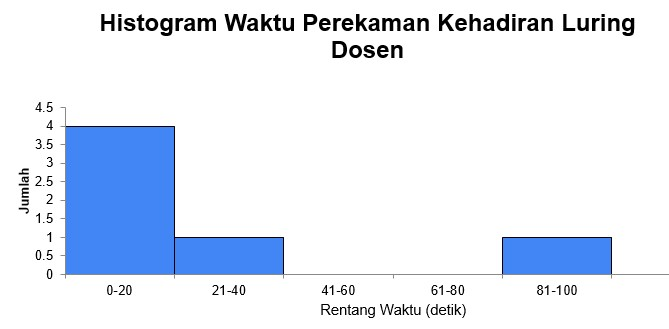
\includegraphics[scale=0.8]{Gambar/LuringDosen.jpg}
		\caption{Histogram Waktu Perekaman Kehadiran Luring Dosen} 
		\label{fig:LuringDosen}
	\end{figure}
	Pada Gambar \ref{fig:LuringDosen} merupakan visualisasi dari hasil survei mengenai lama waktu yang dibutuhkan dari 6 dosen untuk melakukan perekaman kehadiran secara luring. Histogram ini dikelompokan berdasarkan rentang waktu per 20 detik. Histogram menunjukan bahwa sebanyak 4 dosen memiliki rentang waktu 0 sampai 20 detik, 1 dosen memiliki rentang waktu 21 sampai 40 detik, dan 1 dosen memiliki rentang waktu 81 sampai 100 detik. Hasil survei perekeman kehadiran luring untuk setiap dosen secara jelas dapat dilihat pada tabel \ref{tab:luringDosen}.	
	\begin{table}[ht]			
		\caption{Tabel Perekaman Luring Dosen}
		\centering
		\begin{tabular}{|p{4cm} |p{7cm}|}
			\hline
			Jumlah Responden &  Waktu Perekaman Kehadiran Luring \\ \hline     
			1 orang &  1 detik\\ \hline 
			3 orang &  5 detik\\ \hline 
			1 orang &  40 detik\\ \hline 
			1 orang &  90 detik\\ \hline 
		\end{tabular}
		\label{tab:luringDosen}
	\end{table}\\
	Jika dihitung rata-rata waktu yang dibutuhkan untuk melakukan perekaman kehadiran luring bagi para dosen adalah 24,33 detik.
\end{enumerate}
Kesimpulan dari hasil survei dosen menunjukan bahwa rata-rata waktu yang dibutuhkan secara luring adalah 24,33 detik lebih cepat dibandingkan dengan rata-rata waktu yang dibutuhkan secara daring adalah 31,83 detik.
\newpage
\section{Analisis Program Sejenis}
\label{sec:seleniumIDE}  
Selenium IDE merupakan program \textit{open source} untuk otomatisasi di web. Selenium IDE dapat di \textit{install} di browser, contohnya di Google Chrome yang setelah di \textit{install} akan menjadi \textit{extensions}. \textit{Extensions} di Google Chrome adalah sebuah aplikasi kecil yang dapat dijalankan pada Google Chrome itu sendiri. Berikut ini cara untuk melakukan otomatisasi menggunakan Selenium IDE:
	\begin{enumerate}
		\item Membuka Selenium Ide yang tersimpan di \textit{Extensions} pada Google Chrome.
		\item Memilih menu \textit{Record a new test in a new project} (merekam tes baru untuk proyek baru).
		\begin{figure}[H]
			\centering
			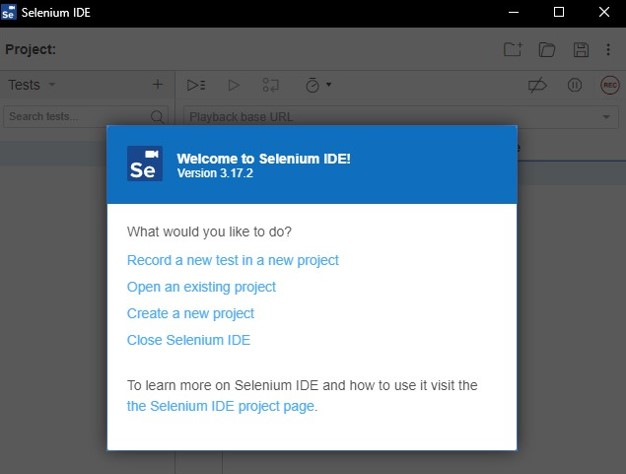
\includegraphics[scale=0.5]{Gambar/menuSeleniumIDE.jpg}
			\caption{Tampilan Menu Awal Selenium IDE} 
			\label{fig:menuSeleniumIDE}
		\end{figure}
		\newpage
		\item Memasukan nama proyek, lalu tekan tombol ``OK''. 
		\begin{figure}[H]
			\centering
			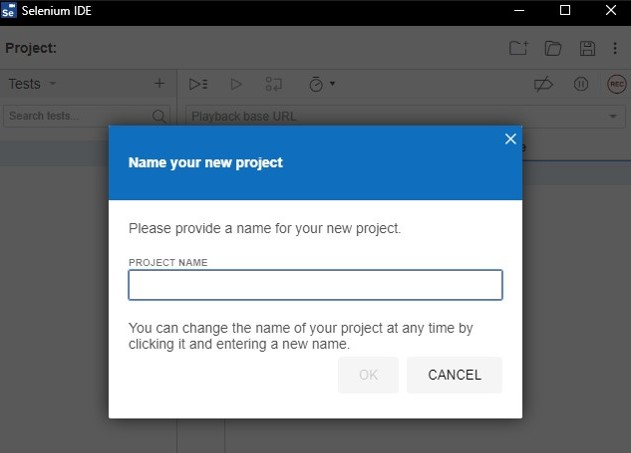
\includegraphics[scale=0.4]{Gambar/namaProyek.jpg}
			\caption{Tampilan Memasukan Nama Proyek} 
			\label{fig:namaProyek}
		\end{figure}
		\item Memasukan situs web, lalu menekan tombol ``START RECORDING''
		\begin{figure}[H]
			\centering
			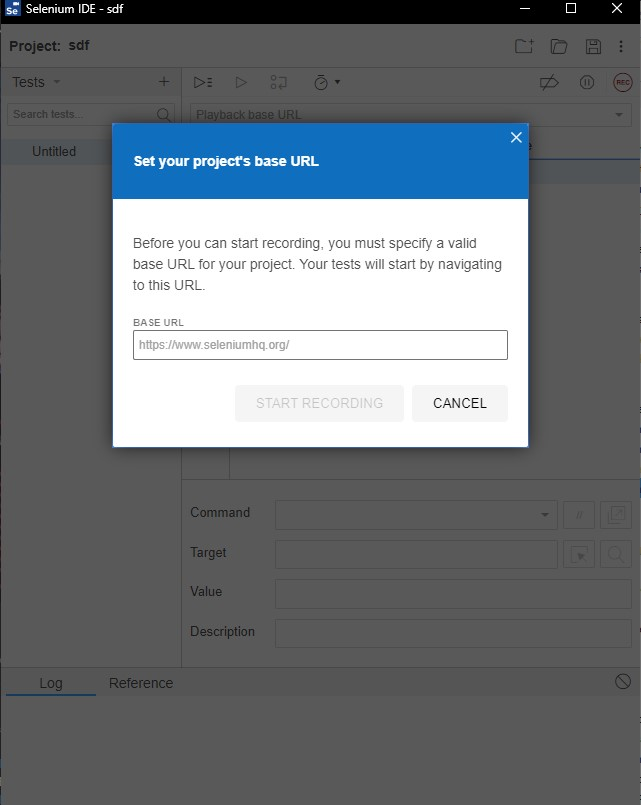
\includegraphics[scale=0.4]{Gambar/baseURL.jpg}
			\caption{Tampilan Memasukan Situs Web} 
			\label{fig:baseURL}
		\end{figure}
		Setelah menekan tombol ``\textit{START RECORDING}'' seperti pada Gambar \ref{fig:baseURL}, maka akan langsung muncul \textit{windows} Google Chrome baru yang langsung menuju situs web yang sudah dimasukan tadi.
		\item Melakukan apa yang ingin diotomatisasikan di \textit{windows} Google Chrome baru yang sudah menuju situs web hingga selesai dan menutup \textit{windows} Google Chrome.
		\begin{figure}[H]
			\centering
			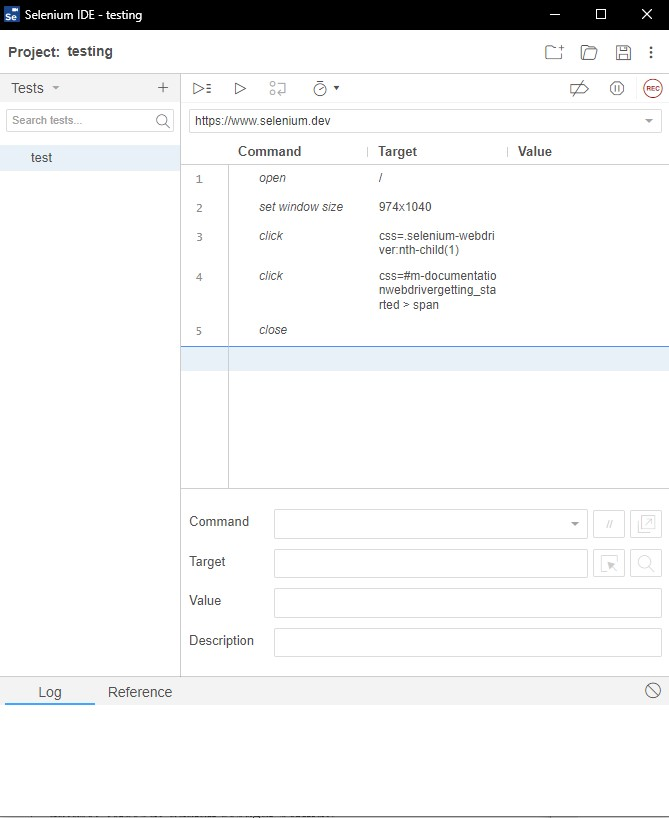
\includegraphics[scale=0.4]{Gambar/testing.jpg}
			\caption{Tampilan Otomatisasi pada Selenium IDE} 
			\label{fig:testing}
		\end{figure}
		Pada Gambar \ref{fig:testing} menunjukan hasil yang sudah terekam dari apa yang sudah dilakukan pada situs web yang ingin diotomatisasikan.
	\end{enumerate}
Selenium IDE ini dapat digunakan untuk melakukan perekaman kehadiran otomatis pada Portal Akademik Mahasiswa. Program yang dibuat pada skripsi ini akan sejenis dengan Selenium IDE, namun program pada skripsi ini akan dapat dijalankan langsung melalui \textit{Command Prompt}. Pada program yang dibuat di skripsi ini membuat pengguna tidak perlu melakukan seperti pada Selenium IDE. Pengguna cukup menjalankan melalui \textit{Command Prompt} saja.